% This will be the main document for the Social Networks paper to
% be written by the Eggnet team of Jordan Ell, Triet Huynh and Braden
% Simpson in association with Adrian Schroeter and Daniela Damian.
\documentclass[conference]{IEEEtran}
\usepackage{graphicx}
\usepackage{amsmath}

% Correct bad hyphenation here
\hyphenation{op-tical net-works semi-conduc-tor}

% Begin the paper here
\begin{document}


% Paper title
% Can use linebreaks \\ within to get better formatting as desired
\title{Changeset Based Developer Communication to Detect Software Failures}

% Authors names
\author{\IEEEauthorblockN{
Braden Simpson}
\IEEEauthorblockA{University of Victoria,
Victoria, British Columbia}
braden@uvic.ca}

% make the title area
\maketitle

\begin{abstract}
As software systems get more complex, the companies developing them consist of larger teams and therefore resulting in more complex communication artifacts.  As these software systems grow, so does the impact of every action to the product.  To prevent software failure created by this growth and complexity, companies need to find out more efficient and effective ways to communicate.  The method used in this paper presents developer communication in the form of social networks of which properties can be used to detect software failures.\end{abstract}

\section{Introduction}

% Setup problem
Miscommunication among contributors during software development can lead to software failures, causing billions of lost dollars or even lethal accidents \cite{Wolf:2009:PBF:1555001.1555017}. Larger products and teams
are inherently complex, making achieving high quality more difficult. To ease this difficulty developers use collaborative development environments (CDE) such as BugZilla, Jira etc. These systems provide bug reports and other communication artifacts which establish a medium for better contributor communication. For this study, we define a \emph{failure-inducing} communication pattern to be a pair of contributors that have a high chance of creating a \emph{fix-inducing change}.  In addition, we define a \emph{changeset} as a set of one or more changes to resources by one developer.  Building social networks, we study the participants and resultant snapshot of the project at that changeset level, to determine if there are any \emph{failure-inducing} patterns of communication present.

% Other research 
In order to create the required networks, we link changesets to communication, similar to Wolf et. al where they link developer networks to build failures\cite{4721184}.  Other researchers such as Bettenburg et al. have done work to link communication artifacts to source code \cite{Bettenburg:2008:ESI:1370750.1370757}.  As well Sliwerski et al. have tried to link fixes(changesets) to their corresponding bug reports \cite{Sliwerski:2005:CIF:1083142.1083147}.  These studies can assist us to understand the direct impact of the communication, and all the effected artifacts.  

% SHOULD reference another section which has the method of making social networks
% Question
We construct social networks on a changeset level over a project's lifetime, and then analyze the history of networks for potential patterns, defined as an unordered pair of contributors of communication.  This drives the question \textit{"Can we identify failure-inducing communication patterns in social networks based on changesets and communications artifacts?"} 

% Method
This paper details our approach at linking social networks to changes, and evaluating their usability for the detection of potentially failure-inducing communication patterns. These include certain problematic groups of participants, or problem areas of a project that require more communication that others due to a more complex technical background.

\section{Approach}
Our goal is to detect potentially failure-inducing patterns in social networks, and in the following sections we describe our methods used to detect these patterns by examining changeset based social networks, resulting in a repository and tool independent process. 

\subsection{Linking Social Data to changesets}
Our goal is to isolate all the communication artifacts that are related to each changeset.  
\subsubsection{Analyzing changeset Message}
First we link by checking the changeset comment for communication related identifiers, usually unique to the specific project. When a strict match to this identifier is found, we construct a link between this changeset and the resulting issue (bug), similar to Sliwerski et al. \cite{Sliwerski:2005:CIF:1083142.1083147}.

\begin{figure}[b!]
\centering
\includegraphics[width=1.0\columnwidth]{CommitsTochangesets1}
\caption{The unique issue identifier found in a changeset comment.\label{fig:identifier}}
\end{figure}

\subsubsection{Parsing Communication Artifacts}
Second, after parsing changeset comments, we use another method to link the communication to source files.  We choose a set of communication artifacts that are within a certain project-specific date-range from the selected changeset.  We continue by parsing the communication artifacts for \textit{Stacktraces, Patches}, and \textit{Code Snippets} using similar methods as Bettenburg et al. \cite{Bettenburg:2008:ESI:1370750.1370757}.  We create confidence of each link based on the percentage of matched content.  This confidence is calculated by taking the ratio of matched code from the code snippet versus the total size of the code snippet. Once the links to files are created, we then check over the changesets that alter those files, and construct a link when one exists.  


% FIX THIS FIGURE to have the definitions of each side
\begin{figure}[t!]
\centering
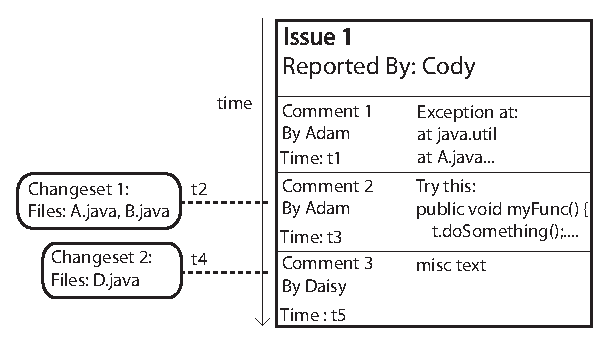
\includegraphics[width=1.0\columnwidth]{Items}
\caption{Timeline of issue, comments and changesets.\label{fig:items}}
\end{figure}

In Figure 2, for example, there are links created between \emph{changeset 1} and \emph{Comment 1}, since there is a \emph{Stacktrace} in \emph{Comment 1} that contains a match to the filename \emph{'A.java'} in \emph{changeset 1}.  This will create a link between artifact and changeset, allowing us to determine the impact of the social network created by these communication artifacts surrounding a changeset.

\subsection{Creating Social Networks} 
Since our goal is to create the networks that are related to a single changeset, our strategy to construct the networks is similar to Wolf et al \cite{4721184}.  The approach taken is repository and tool-independent, and results in networks composed of nodes and edges where the nodes are unique people involved in the communication and the edges are a representation of the communication between those people at the given changeset.  We create these edges like \emph{(Adam, Bart)} where \emph{Adam, Bart} are given by the creators of the artifacts that were linked.   

\subsection{Determining Fix-Inducing Changes}
We qualify each changeset as either a pass or fail, pass meaning that it was a changeset that did not introduce a bug, and conversely a fail is a changeset that introduced a bug.  We used the method from Sliwerski et al \cite{Sliwerski:2005:CIF:1083142.1083147} to infer fix-inducing changes. 

\section{Results}
We used Hibernate-ORM\footnote{An open source Java library that is used for creating object-relational mappings for data-modeling, http://hibernate.org} as a case study.  It is hosted on GitHub, and managed by Jira\footnotemark[2].  Our project requires that both the repository information and the CDE data is able to be mined in order to create the social networks.\\

We classify a failure-inducing pattern by running the statistics through the following formula to calculate the \emph{Failure Index}, FI of a pattern.\\

\begin{equation}
\text{FI} = \frac{\text{pattern}_{failed}/ \text{total}_{failed}}{\text{pattern}_{failed} / \text{total}_{failed} + \text{pattern}_{success} /\text{total}_{success}}
\end{equation}

Before calculating the FI of a pattern, we perform the Fisher Exact Value test to filter out insignificant patterns by selecting only P-Values smaller than \emph{0.05}, then, the significant patterns found with the FI values greater than \emph{0.5} are classified as failure-inducing patterns.  In Table I, we select five failure-inducing patterns, and for those patterns show the number of passing changesets, the number of failing changesets, and the resulting FI.

For the Hibernate-ORM project, which had a total of 3968 changesets, we were able to link 3076 of them to communications artifacts.  From these links, we could create 4537 distinct patterns of communication from the 5040 distinct contributors to the project.  Of those patterns, 178 were significant, and 55 could be identified as failure-inducing. 

\begin{table}[t]
\begin{center}
\begin{tabular}{@{\hspace{.2cm}}ccc@{\hspace{.75cm}}c@{\hspace{.2cm}} l  l  l  l  l }
\hline
Pattern & Passed & Failed & FI & P-Value\\
\hline
(Bob, Drew)	&	0&	3&	1.0000&	0.04910\\
(Carl, Drew)&	0&	3&	1.0000&	0.04910\\
(Alex, Frank)&	19&	25&	0.6947&	0.006908\\
(Frank, Elaine)	&	32&	35&	0.6541&	0.009886\\
(Alex, Elaine)	&	63&	57&	0.6101&	0.01534\\
\hline
\end{tabular}
\end{center}
\caption{Five selected changeset patterns, ordered by Failure Index.\label{tab:ratio}}
\end{table}

\section{Limitations}
One limitation of our study was that we used a large open source project, which means the number of contributors will be a lot larger, but the contributions may be smaller than in closed source projects.   This is reflected heavily in Hibernate, as we had over 5000 contributors, and this resulted in a large amount of insignificant patterns.  

\section{Conclusion and Future Work}
There are several other studies that suggest that better communication practices result in a more successful build rate \cite{Wolf:2009:PBF:1555001.1555017}\cite{Schroter:2010:PBO:1810295.1810456}\cite{4721184}\cite{Zimmermann:2008:PDU:1368088.1368161}, however they perform these studies at a build level, rather than changeset.  Our study suggests that each changeset can be individually analyzed and that failure-inducing patterns of communication (either present or absent) can be extracted.  These patterns can then be used to offer potential recommendations when they are found.  In the future we want to perform another study on a closed source project with a much smaller group of contributors, as the patterns would be more significant, and allow for more analysis. As well, we plan on evaluating the congruence between technical networks and the social networks created in this study to identify other possible failure-inducing patterns. 

\bibliographystyle{IEEEtran}
\bibliography{paper}

% End of the paper
\end{document}

